\documentclass[12pt,letterpaper]{article}
\usepackage[utf8]{inputenc}
\usepackage[spanish]{babel}
\usepackage{graphicx}
\usepackage[left=2cm,right=2cm,top=2cm,bottom=2cm]{geometry}
\usepackage{graphicx} % figuras
% \usepackage{subfigure} % subfiguras
\usepackage{float} % para usar [H]
\usepackage{amsmath}
%\usepackage{txfonts}
\usepackage{stackrel} 
\usepackage{multirow}
\usepackage{enumerate} % enumerados
\renewcommand{\labelitemi}{$-$}
\renewcommand{\labelitemii}{$\cdot$}
% \author{}
% \title{Caratula}
\begin{document}

% Fancy Header and Footer
% \usepackage{fancyhdr}
% \pagestyle{fancy}
% \cfoot{}
% \rfoot{\thepage}
%

% \usepackage[hidelinks]{hyperref} % CREA HYPERVINCULOS EN INDICE

% \author{}
\title{Caratula}

\begin{titlepage}
\begin{center}
\large{UNIVERSIDAD PRIVADA-DE-TACNA}\\
\vspace*{-0.025in}
\begin{figure}[htb]
\begin{center}

\includegraphics[width=8cm]{./Imagenes/logo}
\end{center}
\end{figure}
\vspace*{0.15in}
INGENIERIA DE SISTEMAS  \\

\vspace*{0.5in}
\begin{large}
TITULO:\\
\end{large}

\vspace*{0.1in}
\begin{Large}
\textbf{TRABAJO ENCARGADO No 02} \\
\end{Large}

\vspace*{0.3in}
\begin{Large}
\textbf{CURSO:} \\
\end{Large}

\vspace*{0.1in}
\begin{large}
BASE DE DATOS II\\
\end{large}

\vspace*{0.3in}
\begin{Large}
\textbf{DOCENTE(ING):} \\
\end{Large}

\vspace*{0.1in}
\begin{large}
 Patrick Cuadros Quiroga\\
\end{large}

\vspace*{0.2in}
\vspace*{0.1in}
\begin{large}
Integrantes: \\
\begin{flushleft}
J		\hfill	(201) \\
C 		\hfill	(201) \\
Andre Sebastian Reinoso Aranda          	\hfill	(2016055275) \\
M      	\hfill	(201) \\

\end{flushleft}
\end{large}
\end{center}

\end{titlepage}


\tableofcontents % INDICE
\thispagestyle{empty} % INDICE SIN NUMERO
\newpage
\setcounter{page}{1} % REINICIAR CONTADOR DE PAGINAS DESPUES DEL INDICE

\section{INFORMACIÓN GENERAL} 

\begin{itemize}
\subsection{Objetivos:}
	\item Instalar correctamente una instancia de Microsoft SQL Server.
	\item Conocer fundamentos sobre contenedores.
	\item Aprender comandos basicos de Docker.
\subsection{Equipos, materiales, programas y recursos utilizados:}
	\item Docker Desktop
	\item Microsoft SQL Server 2017 o superior
	\item Virtualización activada en el BIOS.
	\item Windows 10 64bit: Pro, Enterprise o Education, con al menos 4GB de RAM.


\end{itemize}

\section{Nombre del tema} 
Desarrollo

\begin{itemize}
	\item Items
	\\Es correcta
	\begin{center}
	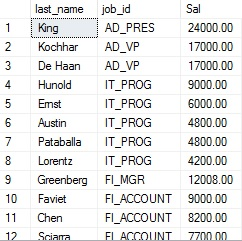
\includegraphics[width=10cm]{./Imagenes/actividad0101} 
	\end{center}



\end{itemize} 
\section{Desarrollo:} 

\begin{itemize}
	\item Crear carpetas
	\\Cree dos carpetas DATALNX DATAWIN

	\begin{center}
	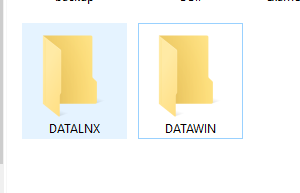
\includegraphics[width=10cm]{./Imagenes/1} 
	\end{center}

\end{itemize} 

\begin{itemize}
	\item Iniciar sesion en docker
	\\Una ves instalado docker y habilitado el Hyper-V, inicie sesion.

	\begin{center}
	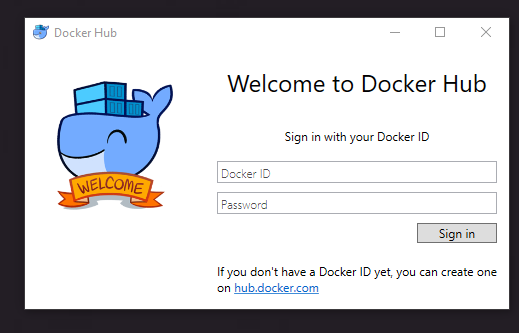
\includegraphics[width=10cm]{./Imagenes/2} 
	\end{center}

\end{itemize} 

\begin{itemize}
	\item PowerShell
	\\Habra el PowerShell con permisos de Administrador.

	\begin{center}
	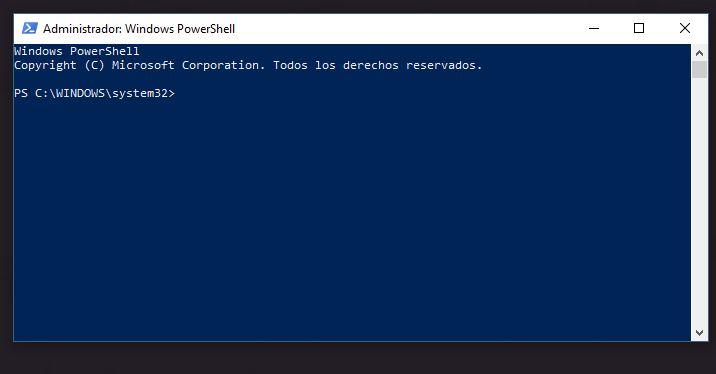
\includegraphics[width=10cm]{./Imagenes/3} 
	\end{center}

\end{itemize} 

\begin{itemize}
	\item Berifica la version de docker
	\\Use el comando "docker version"

	\begin{center}
	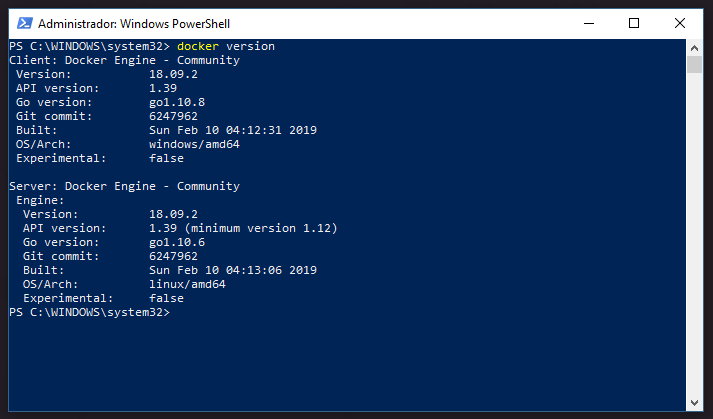
\includegraphics[width=10cm]{./Imagenes/4} 
	\end{center}

\end{itemize} 

\begin{itemize}
	\item Sql en docker
	\\Busque un contenedor con el comando "docker search mssql"

	\begin{center}
	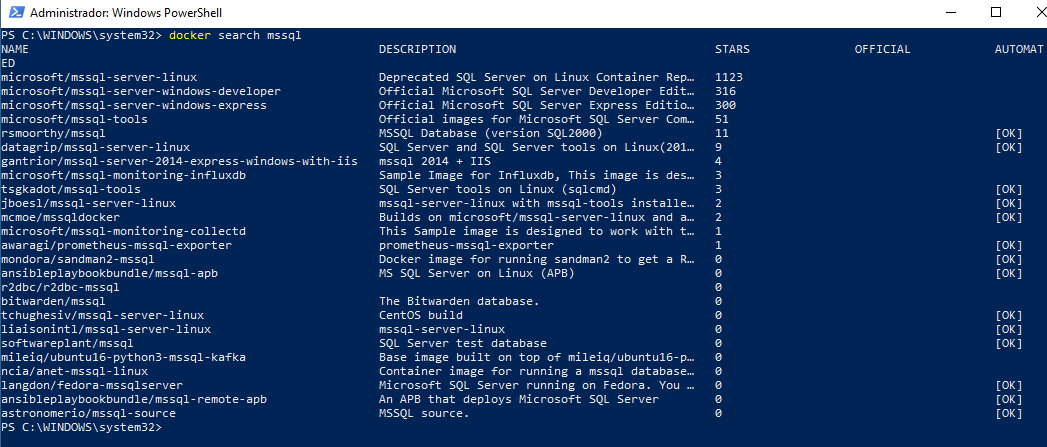
\includegraphics[width=10cm]{./Imagenes/5} 
	\end{center}

\end{itemize} 

\begin{itemize}
	\item Descargar imagen del contenedor
	\\Descargue una imagen con el comando "docker pull microsoft/mssql-server-linux"

	\begin{center}
	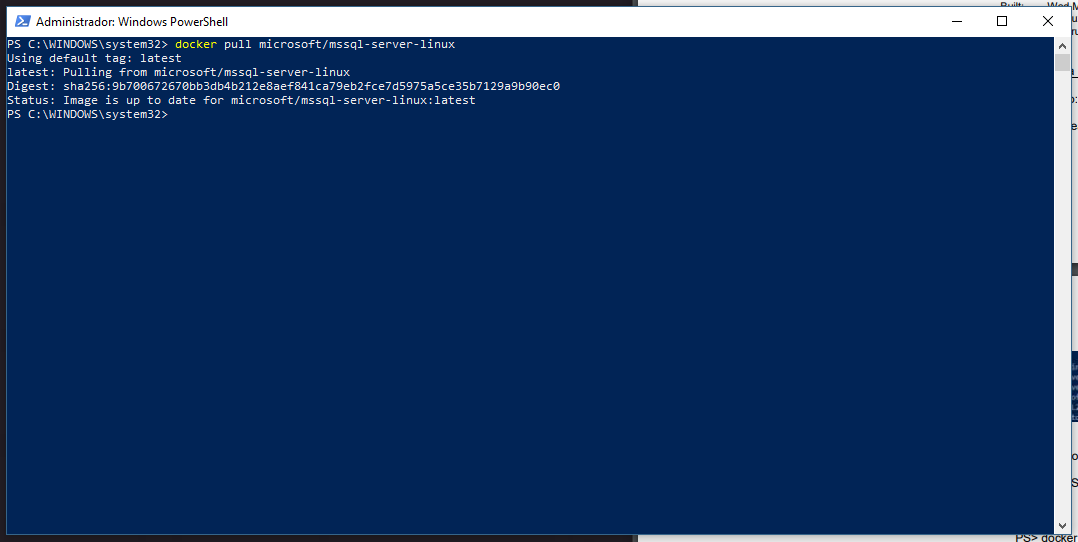
\includegraphics[width=10cm]{./Imagenes/6} 
	\end{center}

\end{itemize}

\begin{itemize}
	\item Verificar
	\\Verifique la imagen con el siguiente comando "docker images"

	\begin{center}
	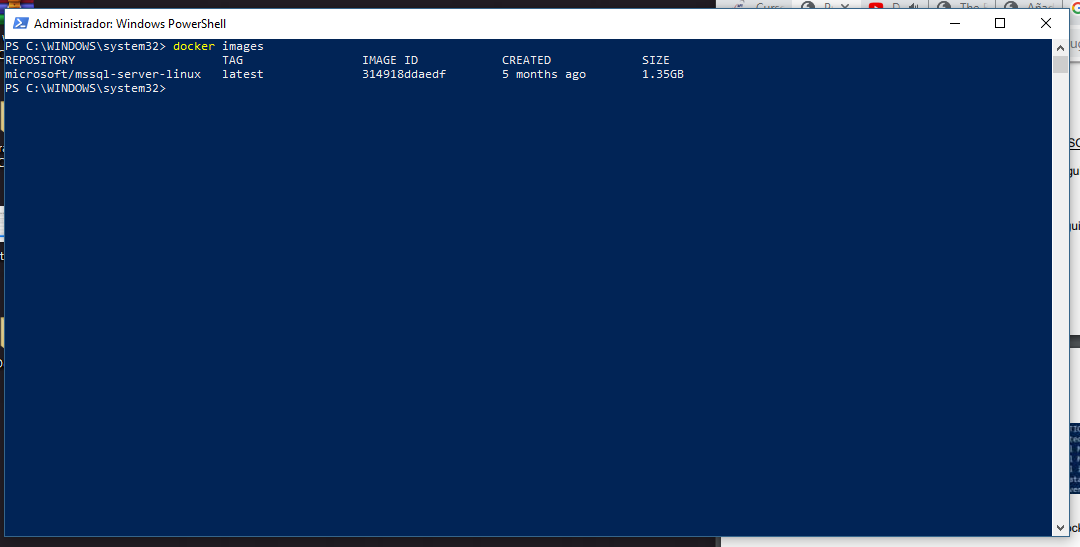
\includegraphics[width=10cm]{./Imagenes/7} 
	\end{center}

\end{itemize} 

\begin{itemize}
	\item Visualizar el ID del contenedor
	\\Usa el comando "docker run ..."

	\begin{center}
	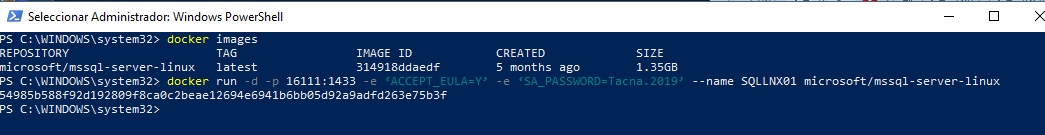
\includegraphics[width=10cm]{./Imagenes/8} 
	\end{center}

\end{itemize} 

\begin{itemize}
	\item Verificar la ejecucion del contenedor
	\\Use el comando "docker ps" para ver el estado del contenedor. Nota: Dar permisos al firewall Windows y aceptelo para realizar la conexion.

	\begin{center}
	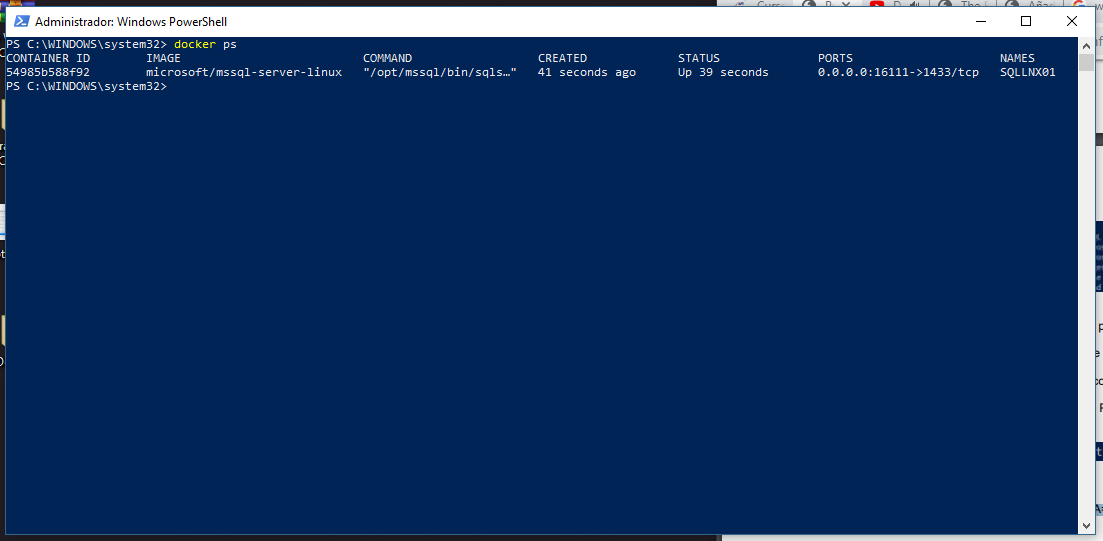
\includegraphics[width=10cm]{./Imagenes/9} 
	\end{center}

\end{itemize} 

\begin{itemize}
	\item Inicie n Microsoft SQL Server Management Studio 
	\\Conectese con los siguientes datos: \textbf{Servidor:}  (local),16111 \textbf{Autenticacion:} SQL Sever \textbf{Usuario:} sa \textbf{Clave:} Tacna.2019

	\begin{center}
	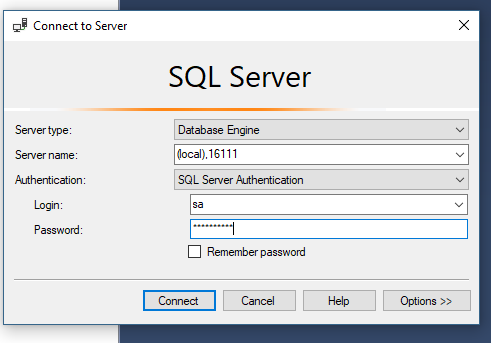
\includegraphics[width=10cm]{./Imagenes/10} 
	\end{center}

\end{itemize} 

\begin{itemize}
	\item Conexion establecida
	\\ Se ve que la conexion fue exitosa

	\begin{center}
	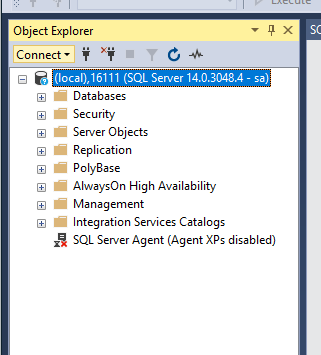
\includegraphics[width=10cm]{./Imagenes/11} 
	\end{center}

\end{itemize} 

\begin{itemize}
	\item Inicie una nueva consulta
	\\Ejecute el siguiente query SELECT @@VERSION

	\begin{center}
	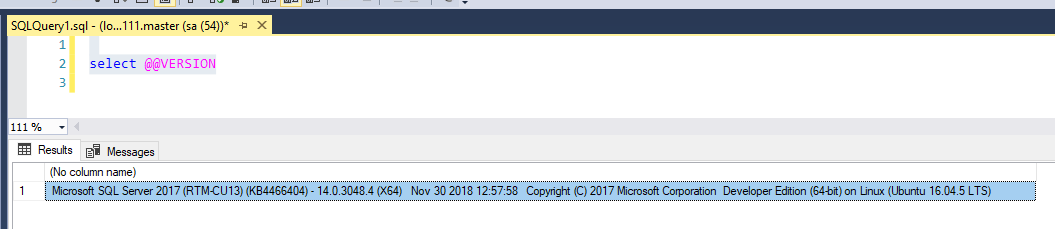
\includegraphics[width=10cm]{./Imagenes/12} 
	\end{center}

\end{itemize} 

\begin{itemize}
	\item Cierre la aplicacion y habra el PowerShell
	\\Para eliminar el contenedor se usa el comando "docker rm -f SQLLNX01", verifique el estado con el comando "docker ps"

	\begin{center}
	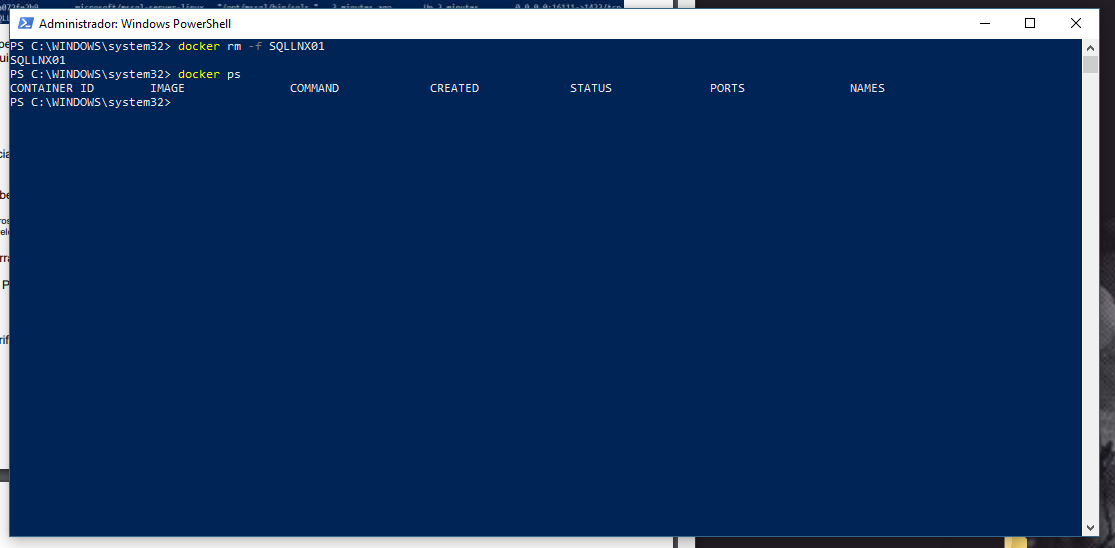
\includegraphics[width=10cm]{./Imagenes/13} 
	\end{center}

\end{itemize} 

\begin{itemize}
	\item Agregando persistencia
	\\Use el comando "docker run ..."

	\begin{center}
	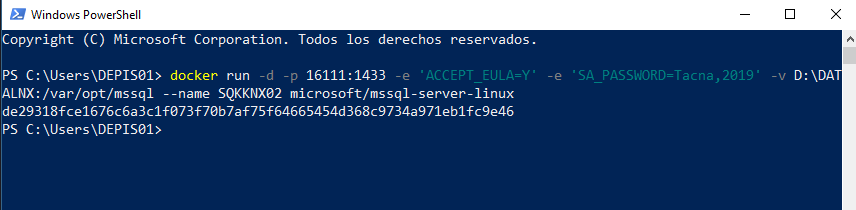
\includegraphics[width=10cm]{./Imagenes/15} 
	\end{center}

\end{itemize} 

\begin{itemize}
	\item Dar permisos
	\\Docker solicitara permisos para guardar los ficheros necesarios

	\begin{center}
	
\includegraphics[width=10cm]{./Imagenes/14} 
	\end{center}

\end{itemize}  

\begin{itemize}
	\item Verifique el status
	\\Use el comando "docker ps"

	\begin{center}
	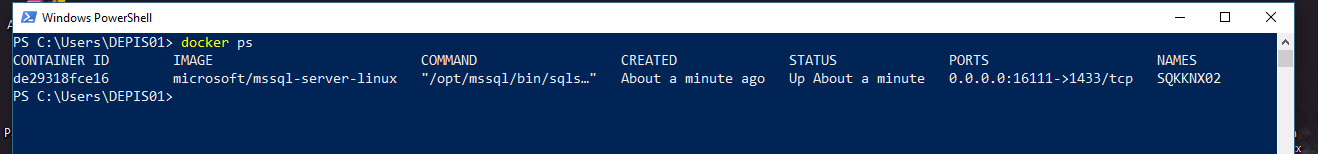
\includegraphics[width=10cm]{./Imagenes/16} 
	\end{center}

\end{itemize} 

\begin{itemize}
	\item Inicie n Microsoft SQL Server Management Studio 
	\\Conectese con los siguientes datos: \textbf{Servidor:}  (local),16111 \textbf{Autenticacion:} SQL Sever \textbf{Usuario:} sa \textbf{Clave:} Tacna.2019

	\begin{center}
	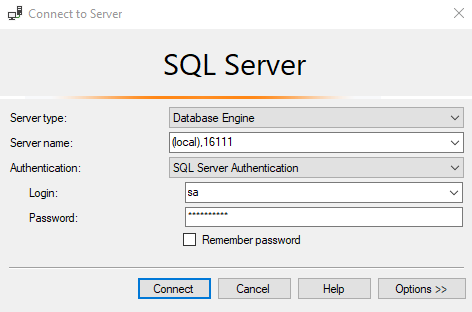
\includegraphics[width=10cm]{./Imagenes/17} 
	\end{center}

\end{itemize} 

\begin{itemize}
	\item Creado una DB
	\\Genere una base de datos a traves del siguiente query

	\begin{center}
	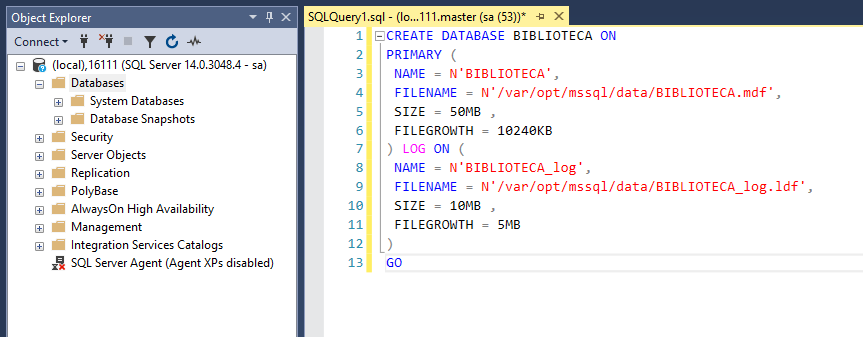
\includegraphics[width=10cm]{./Imagenes/19} 
	\end{center}

\end{itemize} 


\begin{itemize}
	\item Verificarficheros
	\\Abra la carpeta DATALINX y verifique los ficheros y carpetas

	\begin{center}
	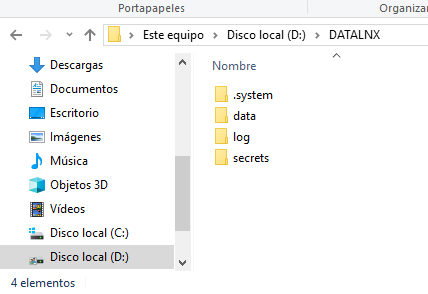
\includegraphics[width=10cm]{./Imagenes/20} 
	\end{center}

\end{itemize} 

\begin{itemize}
	\item Eliminar el contenedor
	\\Use el comando "docker rm -f SQLLNX02"

	\begin{center}
	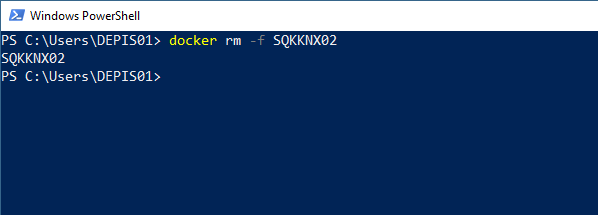
\includegraphics[width=10cm]{./Imagenes/21} 
	\end{center}

\end{itemize} 

\begin{itemize}
	\item Verificando
	\\ Use el comando "docker ps" y verifique que ya no este el contenedor

	\begin{center}
	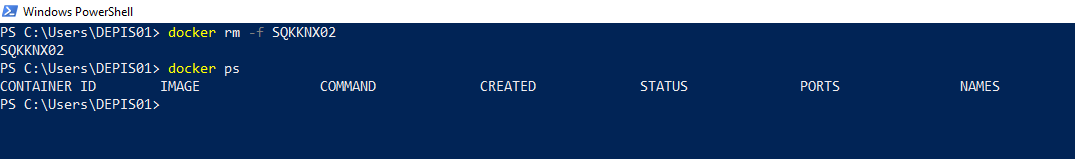
\includegraphics[width=15cm]{./Imagenes/22} 
	\end{center}

\end{itemize} 


\section{Actividades Encargadas} 

\subsection {¿Con qué comando(s) exportaría la imagen de Docker de Microsoft SQL Server a otra PC o servidor?}
\begin{itemize}
	\item El comando usado para exportar es el siguiente:
	
	\begin{center}
	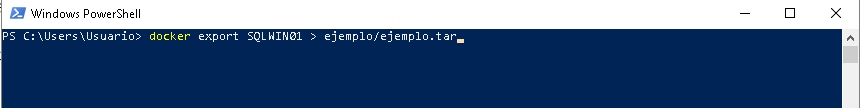
\includegraphics[width=17cm]{./Imagenes/Actividad1} 
	\end{center}

\item De tal modo que se genera un archivor .tar el cual se podra transportar a otra maquina (Windows o Linux).
	\begin{center}
	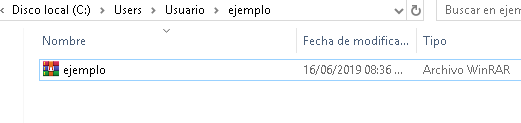
\includegraphics[width=15cm]{./Imagenes/Actividad2} 
	\end{center}
\end{itemize} 
\subsection {¿Con qué comando(s) podría generar dos volúmenes para un contenedor para distribuir en un volumen el Archivo
de Datos (.mdf) y en otro el Archivo Log (.ldf)?}
\begin{itemize}
\item Los comandos para generar dos volúmenes para un contenedor son los siguientes:
\begin{center}
	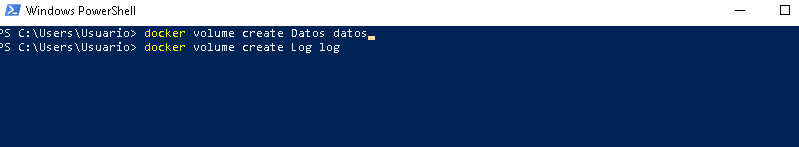
\includegraphics[width=15cm]{./Imagenes/Actividad3} 
	\end{center}
\end{itemize} 

\subsection {Genere un nuevo contenedor y cree la base de datos con las siguientes características.}
\begin{itemize}
\item El Script es:



\begin{center}
	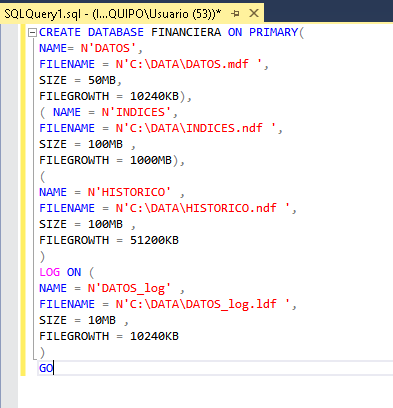
\includegraphics[width=10cm]{./Imagenes/Actividad4} 
	\end{center}

\end{itemize} 
\section{Nombre del tema} 
Desarrollo

\begin{itemize}
	\item Items
	\\Es correcta
	\begin{center}
	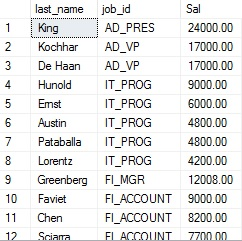
\includegraphics[width=10cm]{./Imagenes/actividad0101} 
	\end{center}



\end{itemize} 
\section{Nombre del tema} 
Desarrollo

\begin{itemize}
	\item Items
	\\Es correcta
	\begin{center}
	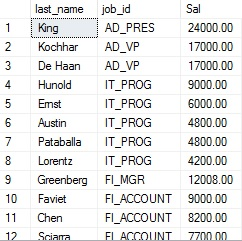
\includegraphics[width=10cm]{./Imagenes/actividad0101} 
	\end{center}



\end{itemize} 
\section{Nombre del tema} 
Desarrollo

\begin{itemize}
	\item Items
	\\Es correcta
	\begin{center}
	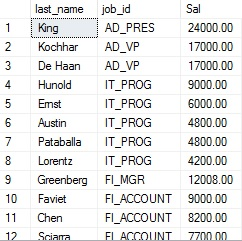
\includegraphics[width=10cm]{./Imagenes/actividad0101} 
	\end{center}



\end{itemize} 
\section{Nombre del tema} 
Desarrollo

\begin{itemize}
	\item Items
	\\Es correcta
	\begin{center}
	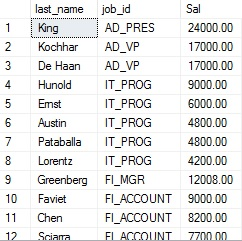
\includegraphics[width=10cm]{./Imagenes/actividad0101} 
	\end{center}



\end{itemize} 
\section{Nombre del tema} 
Desarrollo

\begin{itemize}
	\item Items
	\\Es correcta
	\begin{center}
	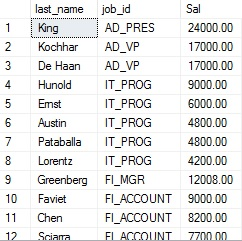
\includegraphics[width=10cm]{./Imagenes/actividad0101} 
	\end{center}



\end{itemize} 
\section{Nombre del tema} 
Desarrollo

\begin{itemize}
	\item Items
	\\Es correcta
	\begin{center}
	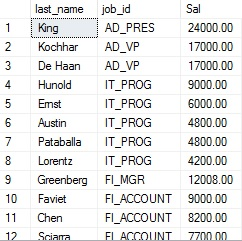
\includegraphics[width=10cm]{./Imagenes/actividad0101} 
	\end{center}



\end{itemize} 

\end{document}
